% 本模板根据中国科学院大学本科生公共必修课程《基础物理实验》Word模板格式编写
% 本模板由Shing-Ho Lin和Jun-Xiong Ji于2022年9月共同完成, 旨在方便LaTeX原教旨主义者和被Word迫害者写实验报告, 避免Word文档因插入过多图与公式造成卡顿. 
% 如有任何问题, 请联系: linchenghao21@mails.ucas.ac.cn
% This is the LaTeX template for experiment report of Experimental Physics courses, based on its provided Word template. 
% This template is completed by the joint collabration of Shing-Ho Lin and Junxiong Ji in September 2022. 
% Adding numerous pictures and equations leads to unsatisfying experience in Word. Therefore LaTeX is better. 
% Feel free to contact us via: linchenghao21@mails.ucas.ac.cn

\documentclass[11pt]{article}

\usepackage[a4paper]{geometry}
\geometry{left=2.0cm,right=2.0cm,top=2.2cm,bottom=2.2cm}

\usepackage{ctex} % 支持中文的LaTeX宏包
\usepackage{amsmath,amsfonts,graphicx,subfigure,amssymb,bm,amsthm,mathrsfs,mathtools,breqn} % 数学公式和符号的宏包集合
\usepackage{algorithm,algorithmicx} % 算法和伪代码的宏包
\usepackage[noend]{algpseudocode} % 算法和伪代码的宏包
\usepackage{fancyhdr} % 自定义页眉页脚的宏包
\usepackage[framemethod=TikZ]{mdframed} % 创建带边框的框架的宏包
\usepackage{fontspec} % 字体设置的宏包
\usepackage{adjustbox} % 调整盒子大小的宏包
\usepackage{fontsize} % 设置字体大小的宏包
\usepackage{tikz,xcolor} % 绘制图形和使用颜色的宏包
\usepackage{multicol} % 多栏排版的宏包
\usepackage{multirow} % 表格中合并单元格的宏包
\usepackage{pdfpages} % 插入PDF文件的宏包
\RequirePackage{listings} % 在文档中插入源代码的宏包
\RequirePackage{xcolor} % 定义和使用颜色的宏包
\usepackage{wrapfig} % 文字绕排图片的宏包
\usepackage{bigstrut,multirow,rotating} % 支持在表格中使用特殊命令的宏包
\usepackage{booktabs} % 创建美观的表格的宏包
\usepackage{circuitikz} % 绘制电路图的宏包
\usepackage[inline]{enumitem}
\usepackage{tabularx}

\usepackage{indentfirst}
\setlength{\parindent}{2em}
\setlength{\abovecaptionskip}{2pt}
\setlength{\belowcaptionskip}{2pt}
\setlength{\intextsep}{8pt}
\setlength{\floatsep}{8pt}

\definecolor{dkgreen}{rgb}{0,0.6,0}
\definecolor{gray}{rgb}{0.5,0.5,0.5}
\definecolor{mauve}{rgb}{0.58,0,0.82}
\lstset{
  frame=tb,
  aboveskip=3mm,
  belowskip=3mm,
  showstringspaces=false,
  columns=flexible,
  framerule=1pt,
  rulecolor=\color{gray!35},
  backgroundcolor=\color{gray!5},
  basicstyle={\small\ttfamily},
  numbers=none,
  numberstyle=\tiny\color{gray},
  keywordstyle=\color{blue},
  commentstyle=\color{dkgreen},
  stringstyle=\color{mauve},
  breaklines=true,
  breakatwhitespace=true,
  tabsize=3,
}

% 轻松引用, 可以用\cref{}指令直接引用, 自动加前缀. 
% 例: 图片label为fig:1
% \cref{fig:1} => Figure.1
% \ref{fig:1}  => 1
\usepackage[capitalize]{cleveref}
% \crefname{section}{Sec.}{Secs.}
\Crefname{section}{Section}{Sections}
\Crefname{table}{Table}{Tables}
\crefname{table}{Table.}{Tabs.}

\setmainfont{Palatino Linotype.ttf}
\setCJKmainfont{SimHei.ttf}
% \setCJKsansfont{Songti.ttf}
% \setCJKmonofont{SimSun.ttf}
\punctstyle{kaiming}
% 偏好的几个字体, 可以根据需要自行加入字体ttf文件并调用

\renewcommand{\emph}[1]{\begin{kaishu}#1\end{kaishu}}

%改这里可以修改实验报告表头的信息
\newcommand{\experiName}{弦上驻波及介质中声速测量}
\newcommand{\supervisor}{吴天涯}
\newcommand{\name}{张欣培}
\newcommand{\studentNum}{2022K8009922001}
\newcommand{\class}{01}
\newcommand{\group}{10}
\newcommand{\seat}{9}
\newcommand{\dateYear}{2023}
\newcommand{\dateMonth}{12}
\newcommand{\dateDay}{18}
\newcommand{\room}{教721}
\newcommand{\others}{$\square$}
%% 如果是调课、补课, 改为: $\square$\hspace{-1em}$\surd$
%% 否则, 请用: $\square$
%%%%%%%%%%%%%%%%%%%%%%%%%%%

\begin{document}

%若需在页眉部分加入内容, 可以在这里输入
% \pagestyle{fancy}
% \lhead{\kaishu 测试}
% \chead{}
% \rhead{}

\begin{center}
    \LARGE \bf 《\, 基\, 础\, 物\, 理\, 实\, 验\, 》\, 实\, 验\, 报\, 告
\end{center}

\begin{center}
    \noindent \emph{实验名称}\underline{\makebox[25em][c]{\experiName}}
    \emph{指导教师}\underline{\makebox[8em][c]{\supervisor}}\\
    \emph{姓名}\underline{\makebox[6em][c]{\name}} 
    % 如果名字比较长, 可以修改box的长度"6em"
    \emph{学号}\underline{\makebox[10em][c]{\studentNum}}
    \emph{分班分组及座号} \underline{\makebox[5em][c]{\class \ -\ \group \ -\ \seat }\emph{号}} (\emph{例}:\, 1\,-\,04\,-\,5\emph{号})\\
    \emph{实验日期} \underline{\makebox[3em][c]{\dateYear}}\emph{年}
    \underline{\makebox[2em][c]{\dateMonth}}\emph{月}
    \underline{\makebox[2em][c]{\dateDay}}\emph{日}
    \emph{实验地点}\underline{{\makebox[4em][c]\room}}
    \emph{调课/补课} \underline{\makebox[3em][c]{\others\ 是}}
    \emph{成绩评定} \underline{\hspace{5em}}
    {\noindent}
    \rule[8pt]{17cm}{0.2em}
\end{center}

\begin{center}
    \Large \bf 第一部分\qquad 实验内容
\end{center}

\section{实验目的}

\begin{enumerate}
    \item 观察在两端固定的弦线上形成的驻波现象,了解弦线达到共振和形成稳定驻波的条件;
    \item 测定弦线上横波的传播速度;
    \item 用实验的方法确定弦线作受迫振动时共振频率与半波长个数n、弦线有效长度、张力及弦密度之间的关系;
    \item 用对数作图和最小乘法对共振频率与张力关系的实验结果作线性拟合,处理数据,并给出结论。
\end{enumerate}

\section{实验器材}

    \hspace*{2em} 弦音计、信号发生器、双踪示波器、天平(高精度,低精度)SW-2型声速测量仪。
\begin{figure}[H]
    \centering
    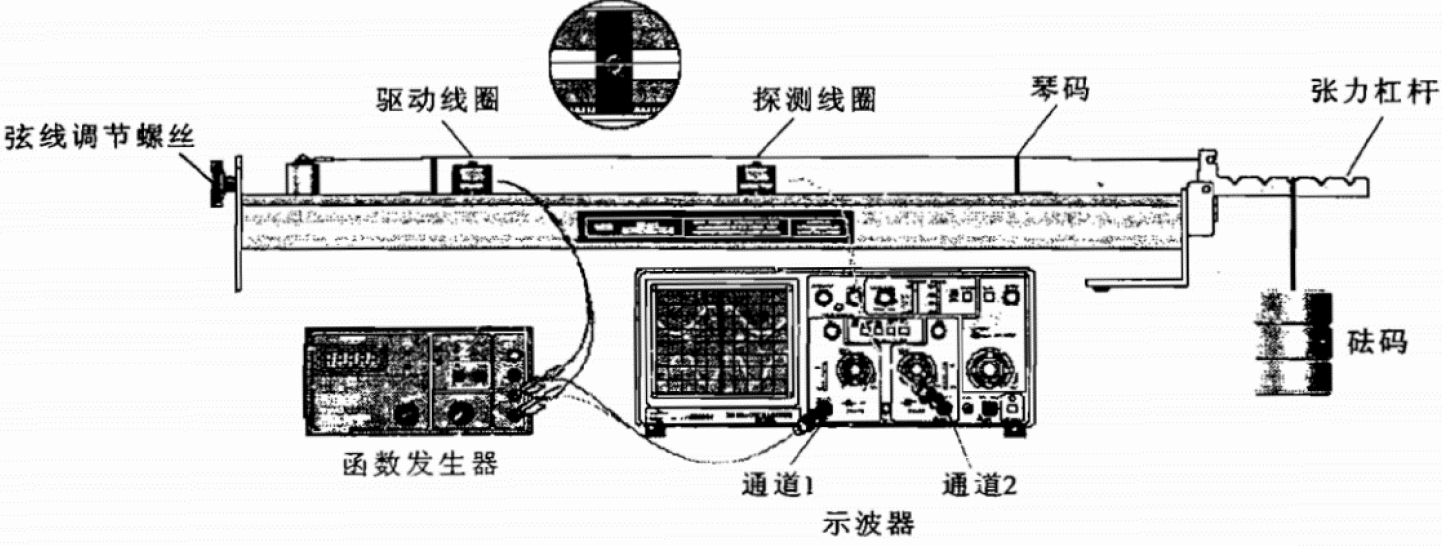
\includegraphics[width=12cm]{Fig/1.png}
    \caption{弦音计}
\end{figure}
\begin{figure}[H]
    \centering
    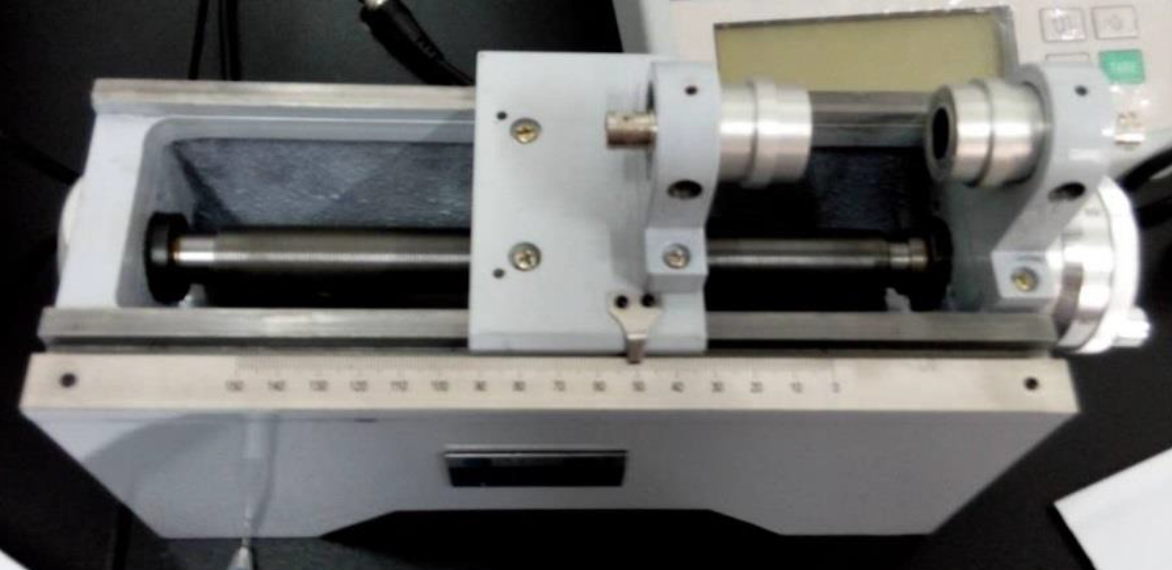
\includegraphics[width=10cm]{Fig/1.5.png}
    \caption{声速测量仪}
\end{figure}
\section{实验原理}

\begin{enumerate}
    \item 驻波
    \par 简谐波的方程为:
    \begin{equation}
        y=A\cos\left(\omega t-kx+\varphi\right)
    \end{equation}
    其中,$k=\frac{2\pi}{\lambda}$是角波数,$\lambda$是波长。两列振幅、频率相同,方向相反的简谐波合成时,
    \begin{equation}
        y_1+y_2=2A\cos\left(kx+\frac{\varphi_2-\varphi_1}{2}\right)\cos\left(\omega t+\frac{\varphi_2+\varphi_1}{2}\right)
    \end{equation}
    对于同一位置x,最大振幅为
    \begin{equation}
        A(x)=\left|2A\cos\left(kx+\frac{\varphi_2-\varphi_1}{2}\right)\right|
    \end{equation}
    对于振幅为最大振幅2A的点称为波腹,对于振幅为最小振幅0的点称为波节。
    \\波腹的位置为:
    \begin{equation}
        x=\pm\frac{n}{2}\lambda \mp\frac{\varphi_2-\varphi_1}{2k}\qquad n=0,\pm1,\pm2...
    \end{equation}
    波节的位置为:
    \begin{equation}
        x=\pm\frac{n+\frac{1}{2}}{2}\lambda \mp\frac{\varphi_2-\varphi_1}{2k}\qquad n=0,\pm1,\pm2...
    \end{equation}
    相邻两波腹或两波节之间的间距$D=\frac{\lambda}{2}$,称为半波长。
    \\从观察上,驻波的特点是点看起来在原地震动,而不是向前传递。
    \item 弦上驻波及其特性
    \par \hspace*{2em}要观察稳定的驻波,须具备两个条件:1)波长易于观察且频率较稳定,传播介质要稳定不
    易受到干扰;2)传播方向相反的两列波相干,即频率和振幅均相同,并具有固定的相位差。本
    实验选用两端固定且紧绷的琴弦作为传播介质,利用在弦上传播的机械波及其反射波产生驻波。
    \\\hspace*{2em}本实验中,在弦上一点有策动源,其在两个端点的一次或多次反射波与原来的波进行合成形成驻波。由于半波损失的存在,反射波与反射前的一列波的频率和振幅相同,方向相反,而相位总是相差$\pi$。
    \\\hspace*{2em}驻波的频率就是输入波的频率$f=\frac{\omega}{2\pi}=\frac{kv}{2\pi}$,其中$v$是入射波波速。当弦长为L,且恰好为半波长D的整数倍时,有稳定的驻波,此时$f=n\frac{v}{2L}$。$n=1$时,称为弦的基频$f_1=\frac{v}{2L}$。弦的共振频率是基频的整数倍,$f_n=nf_1$。
    \\\hspace*{2em}对于一段拉紧弦的张力为$T$,线密度为$\mu$的琴弦,通过波的运动方程
    \begin{equation}
        \begin{split}
            \frac{\partial^2y}{\partial t^2}=\frac{T}{\mu}\frac{\partial^2y}{\partial x^2} \\
            \frac{\partial^2y}{\partial t^2}=v^2\frac{\partial^2y}{\partial x^2}
        \end{split}
    \end{equation}
    解得$v=\sqrt{\frac{T}{\mu}}$,则共振频率(基频)为:
    \begin{equation}
        f_1=\frac{1}{\lambda}\sqrt{\frac{T}{\mu}}
    \end{equation}
    对等式两边取对数,有
    \begin{equation}{\label{equ:8}}
        \log f_1=\frac{1}{2}\log T-\frac{1}{2}\log \mu-\log \lambda
    \end{equation}
    \item 驻波共振频率的判断与观察
    \par \hspace*{2em}在示波器上,驻波在共振频率时振幅极大,也许琴弦会有明显的声音。示波器观察波形振幅时误差较大,因此频率调整区间没必要太小,精确到$0.1Hz$即可。
\end{enumerate}


\section{实验内容}
\subsection{线密度测试}
\noindent 实验步骤:
\begin{enumerate}
    \item 取样品弦,记录弦号。
    \item 用高精度天平测样品弦质量m。
    \item 用直尺测样品弦长度l(由于弦弯曲难以测量长度,不进行估读)。
    \item 用螺旋测微器测样品弦直径d。
    \item 由$\mu=\frac{m}{l}$计算线密度。
\end{enumerate}
\noindent 实验数据:
\begin{table}[H]
    \centering
    \caption{线密度测试}
    \begin{tabular}{|c|c|c|c|c|}
    \hline
        弦号 & 质量(g) & 长度(mm) & 直径(mm) & 线密度(kg/m) \\ \hline
        9 & 0.199 & 9.7 & 0.651 & 2.05E-03 \\ \hline
    \end{tabular}
\end{table}
\subsection{波速的测量}
\noindent 实验步骤:
\begin{enumerate}
    \item 将低精度天平调零,测砝码质量M。
    \item 将琴码放在150mm和650mm的地方,将砝码放在第2-4格,测基频$f_1$,倍频$f_2,f_3$,计算波速的实验值($v=\lambda f$),根据$v=\sqrt{\frac{T}{\mu}}$,$T=\frac{1}{2}nmg$计算波速的理论值。取$g=9.8m/s^2$
\end{enumerate}
\begin{figure}[H]
    \centering
    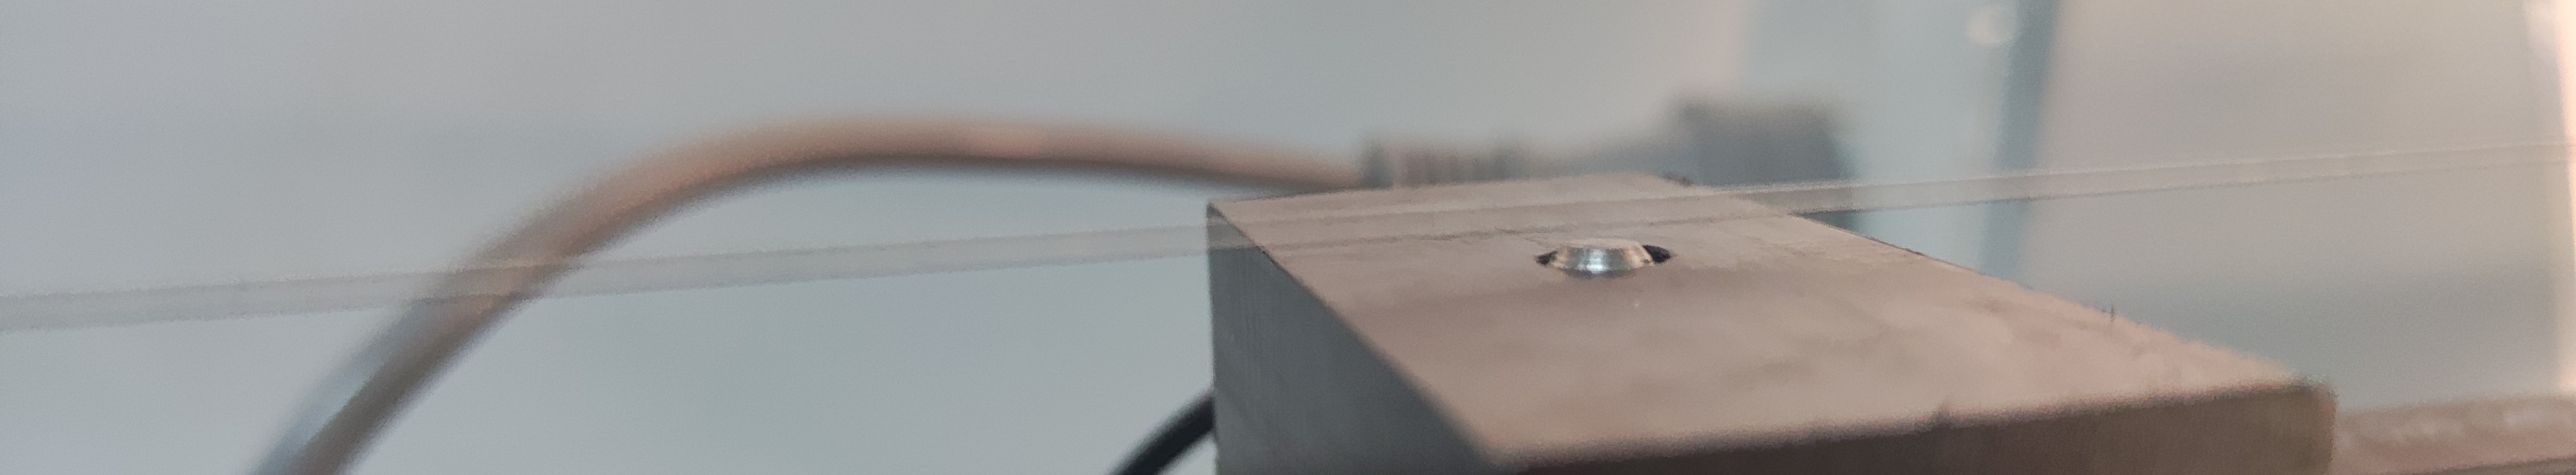
\includegraphics[width=14cm]{Fig/2.jpg}
    \caption{驻波}
\end{figure}
\noindent 实验数据:
\\砝码质量:505.78g
\begin{table}[H]
    \centering
    \caption{波速的测试}
    \begin{tabular}{|c|c|c|c|c|c|c|}
    \hline
        砝码位置 & $f_1/Hz$ & $f_2/Hz$ & $f_3/Hz$ & 波速测量值$v/(m/s)$ & $T/N$ & 波速计算值$v/(m/s)$ \\ \hline
        2 & 52.5 & 105.2 & 157.8 & 52.5 & 4.957  & 49.17  \\ \hline
        3 & 60.6 & 121.3 & 181.7 & 60.6 & 7.435  & 60.22  \\ \hline
        4 & 67.3 & 134.7 & 204.6 & 67.3 & 9.913  & 69.54 \\ \hline
    \end{tabular}
\end{table}
最大实验误差$\frac{52.5-49.17}{49.17}=6.8\%$。经过最小二乘法计算,$T=k\cdot nmg$系数$k=0.4999\approx0.5$,误差可忽略。
\subsection{共振频率和有效长度的关系}
\noindent 实验步骤:
\begin{enumerate}
    \item 将砝码放在第二个,改变琴码位置以改变有效长度,测量共振频率(基频)$f_1$。
\end{enumerate}
\noindent 实验数据:
\begin{table}[H]
    \centering
    \caption{频率和有效长度的关系}
    \begin{tabular}{|c|c|c|c|c|c|}
    \hline
        $L/mm$ & 640 & 480 & 320 & 240 & 160 \\ \hline
        $f_1/Hz$ & 36.7 & 52.5 & 83.8 & 113.1 & 161.2 \\ \hline
        $\frac{1}{\lambda}=\frac{1}{2L}/m^{-1}$ & 0.781  & 1.04   & 1.56   & 2.08   & 3.12 \\\hline
    \end{tabular}
\end{table}
\begin{figure}[H]
    
\end{figure}
由\cref{fig:3}图像拟合可以看出,$f$-$\lambda$图像为线性图,$f\cdot \lambda$应为常数,即波速v。拟合图像后得$v=53.34m/s$,与理论值偏差$\frac{53.34-49.17}{49.17}=8.5\%$。

\begin{figure}[H]
    \centering
    \begin{minipage}[t]{0.49\linewidth}
        \centering
        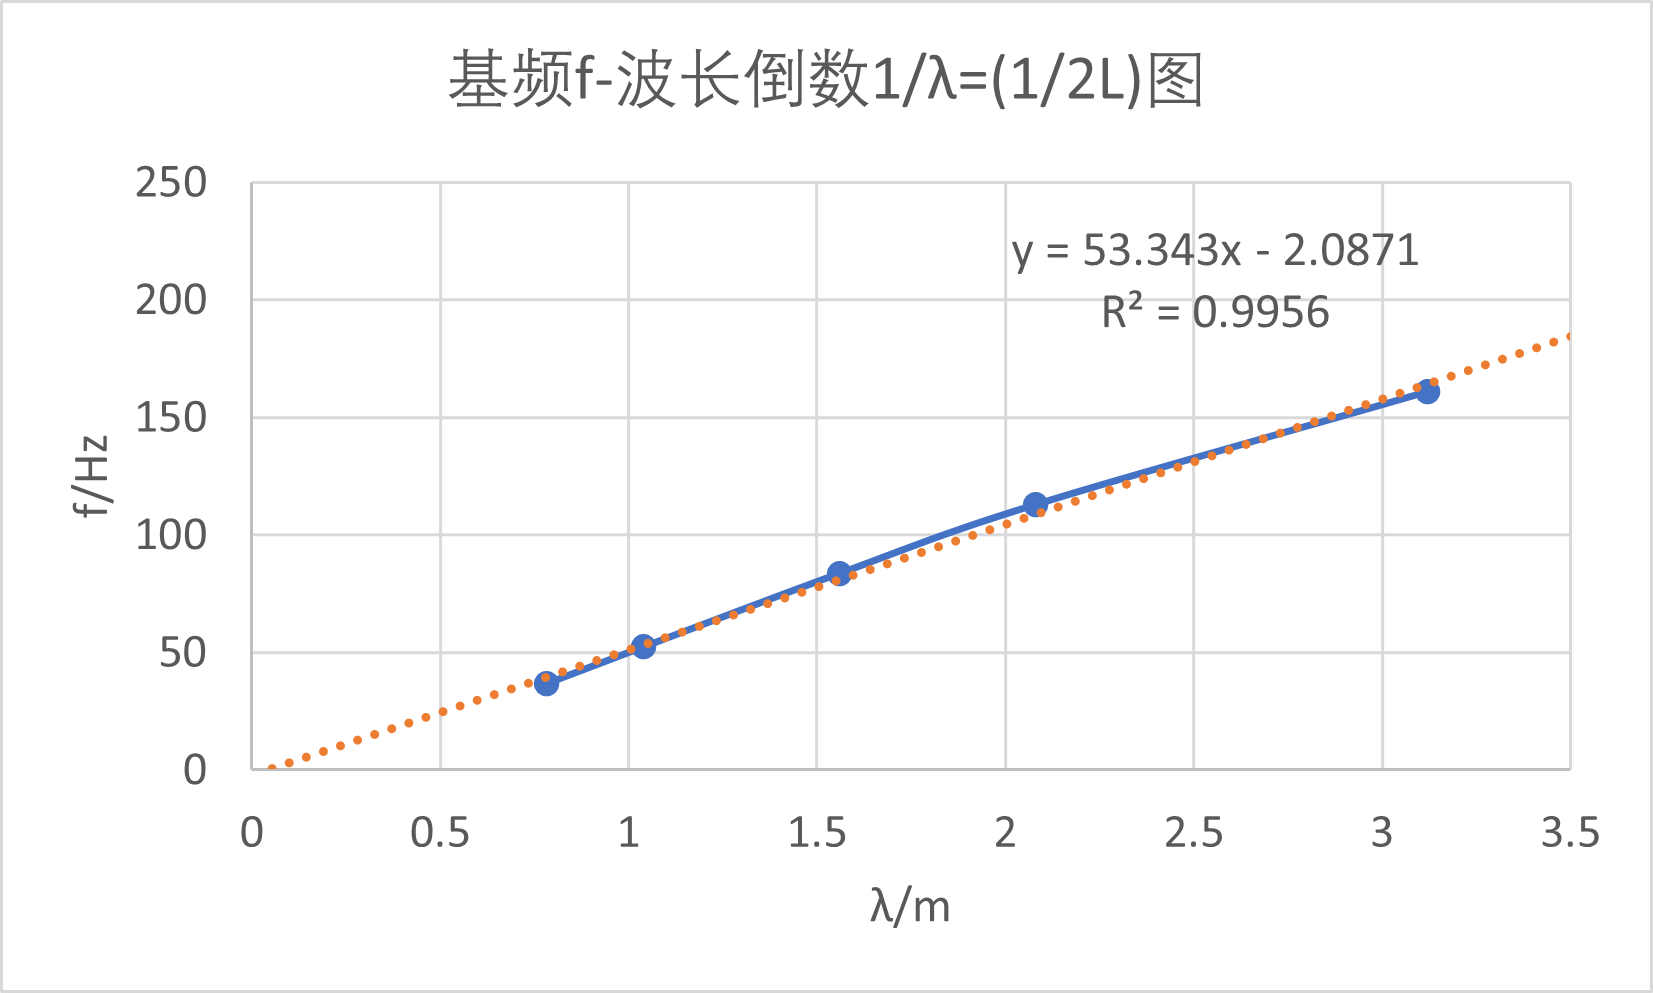
\includegraphics[width=7.7cm]{Fig/3.png}
        \caption{f-$\frac{1}{\lambda}$图}
        \label{fig:3}
    \end{minipage}
    \begin{minipage}[t]{0.49\linewidth}
        \centering
        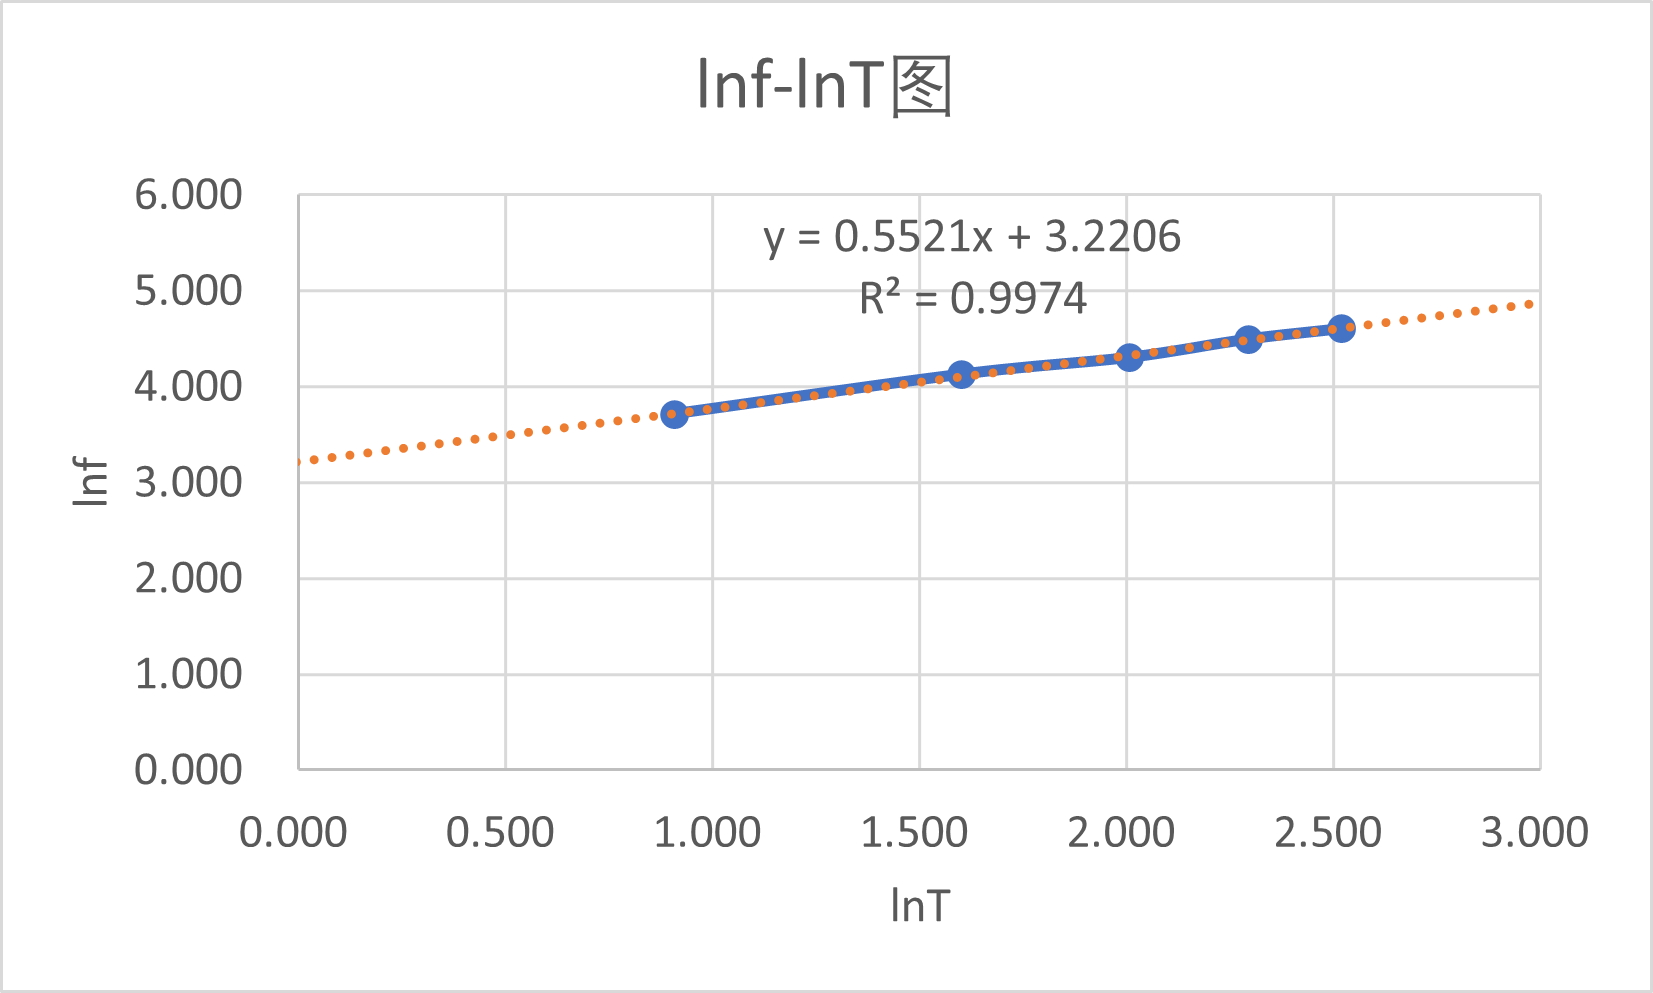
\includegraphics[width=7.7cm]{Fig/4.png}
        \caption{$\ln f_1$-$\ln T$图}
        \label{fig:4}
    \end{minipage} 
\end{figure}
\subsection{共振频率和张力的关系}
\noindent 实验步骤:
\begin{enumerate}
    \item 调整琴码,固定有效长度$L=400mm$,将琴码放在200mm和600mm的地方。
    \item 将砝码放在1-5格,测量$f_1$。
\end{enumerate}
\noindent 实验数据:
\begin{table}[H]
    \centering
    \caption{频率和张力的关系}
    \begin{tabular}{|c|c|c|c|c|c|}
    \hline
        位置 & 1 & 2 & 3 & 4 & 5 \\ \hline
        $T/N$ & 2.48  & 4.96  & 7.43  & 9.91  & 12.39  \\ \hline
        $f_1/Hz$ & 41.0  & 62.1  & 74.1  & 89.8  & 100.1  \\ \hline
        $\ln T$ & 0.908  & 1.601  & 2.006  & 2.294  & 2.517  \\ \hline
        $\ln f_1$ & 3.714  & 4.129  & 4.305  & 4.498  & 4.606 \\ \hline
    \end{tabular}
\end{table}
    由\cref{fig:4}图像拟合,$\ln f=0.552\ln T+3.220$。和公式\eqref{equ:8}相比,斜率误差$10.4\%$,原公式截距$-\frac{1}{2}\log \mu-\log \lambda=3.318$,截距误差$3.0\%$。

\subsection{共振频率和线密度的关系}
\noindent 实验步骤:
\begin{enumerate}
    \item 调整琴码,固定有效长度$L=400mm$,将琴码放在200mm和600mm的地方。
    \item 将砝码放在第2格,测量$f_1$。(可取其他同学的数据,不用自己测量)
\end{enumerate}
\noindent 实验数据:
\begin{table}[H]
    \centering
    \caption{频率和线密度的关系}
    \begin{tabular}{|c|c|c|c|c|c|}
    \hline
        弦号 & 10 & 8 & 5 & 11 & 7 \\ \hline
        直径/mm & 1.192  & 1.042  & 1.396  & 0.890  & 0.824  \\ \hline
        μ/(kg/m) & 7.32E-03 & 5.50E-03 & 3.75E-03 & 3.70E-03 & 3.37E-03 \\ \hline
        f1/Hz & 32.6 & 39.89 & 46.38 & 47.53 & 48.93 \\ \hline
        lnf1 & 3.4843  & 3.6861  & 3.8369  & 3.8614  & 3.8904  \\ \hline
        lnμ & -4.9171  & -5.2030  & -5.5860  & -5.5994  & -5.6928 \\ \hline
    \end{tabular}
\end{table}
\begin{figure}[H]
    \centering
    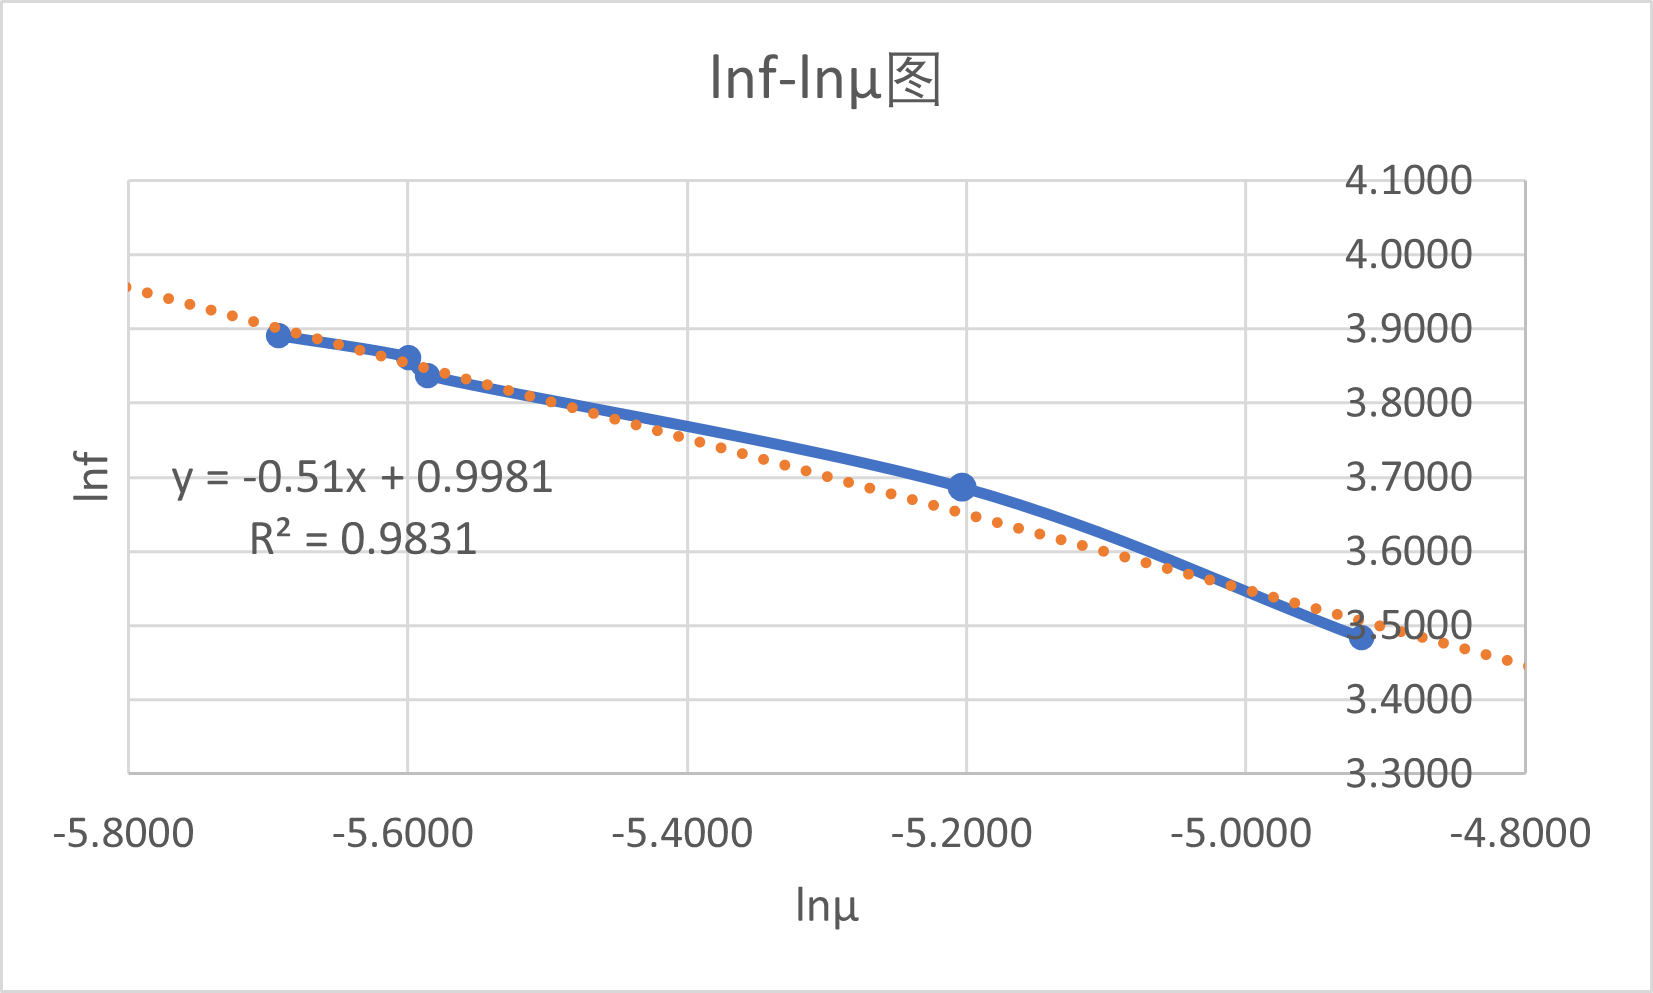
\includegraphics[width=8cm]{Fig/5.png}
    \caption{$\ln f_1$-$\ln \mu$图}
\end{figure}
\par 可以看到,拟合直线后$\ln f_1=-0.51\ln \mu+0.9981$。和公式\eqref{equ:8}相比,斜率误差$2\%$;按$T=0.5*505g*2*9.8m/s^2=4.95N$计算,原式截距$\frac{1}{2}\log T-\log \lambda=1.023$,截距误差$2.4\%$。由于使用的砝码不一,实际上T并不唯一,直线拟合时按单变量拟合也会有问题。
\subsection{测超声波在空气和水中的波速}
\noindent 实验步骤:
\begin{enumerate}
    \item 在超声波测量仪上安装超声信号发射端(接收端),连接到示波器上。
    \item (驻波法)扭动旋钮,测示波器上振幅极大时的位置,测10组。
    \item (位相法)使用示波器X-Y模式,测李萨如图像改变半个周期/一个周期时的位置,测10组。
    \begin{figure}[H]
        \centering
        \begin{minipage}[t]{0.25\linewidth}
            \centering
            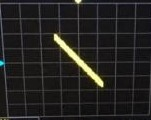
\includegraphics[width=3.7cm]{Fig/fake.jpg}
            \caption{示波器上李萨如图像}
        \end{minipage}
        \begin{minipage}[t]{0.74\linewidth}
            \centering
            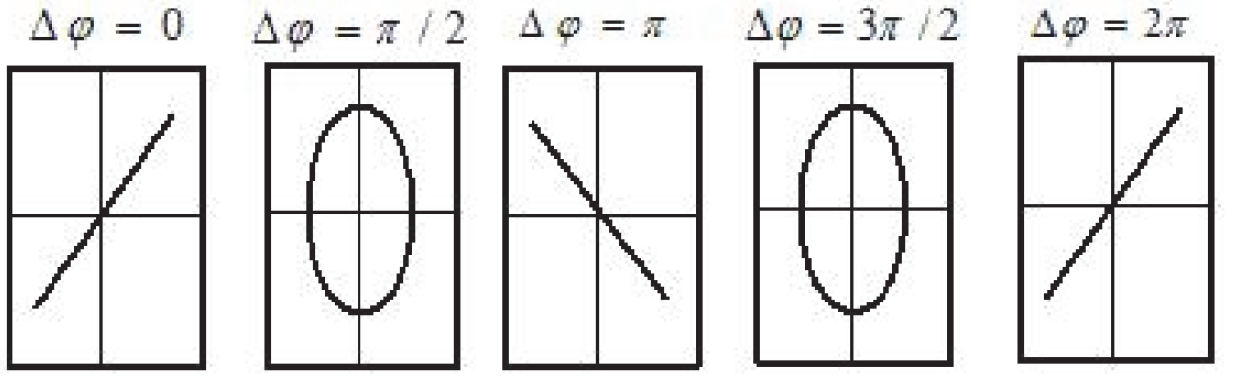
\includegraphics[width=12cm]{Fig/6.png}
            \caption{李萨如图像参考}
        \end{minipage} 
    \end{figure}
    \item 用逐差法处理数据。
\end{enumerate}
\noindent 实验数据:
\par \noindent 空气中波速:\quad$f=40kHz$,\qquad 室温$t=23.1^\circ C$,\qquad $v_{\text{理论值}}=v_0\sqrt{\frac{T}{T_0}}=331.45\times \sqrt{\frac{273.15+23.1}{273.15}}=345.18(m/s)$
\begin{table}[H]
    \centering
    \caption{空气中超声波波速的测试}
    \begin{tabular}{|c|c|c|c|c|}
    \hline
        i & 驻波法$L_i/mm$ & $\lambda_i$ & 位相法$L_i/mm$ & $\lambda_i$ \\ \hline
        1 & 15.809  & 23.612  & 16.030  & 21.940  \\ \hline
        2 & 21.249  & 22.113  & 21.475  & 20.799  \\ \hline
        3 & 24.970  & 23.344  & 25.990  & 20.358  \\ \hline
        4 & 29.998  & 22.902  & 29.254  & 21.399  \\ \hline
        5 & 34.772  & 23.548  & 33.851  & 22.507  \\ \hline
        6 & 39.421  & ~ & 37.970  & ~ \\ \hline
        7 & 43.362  & ~ & 42.274  & ~ \\ \hline
        8 & 48.314  & ~ & 46.348  & ~ \\ \hline
        9 & 52.900  & ~ & 50.653  & ~ \\ \hline
        10 & 58.320  & ~ & 56.358 & ~ \\ \hline
    \end{tabular}
\end{table}

\par 本部分实验中,每次移动半个波长。在驻波法中,由逐差法,半波长$\frac{\lambda}{2}=4.621(mm)$,$v=\lambda f=369.68(m/s)$,误差$7.1\%$。位相法中,由逐差法,半波长$\frac{\lambda}{2}=4.280(mm)$,$v=\lambda f=342.40(m/s)$,误差$0.8\%$。位相法误差远远小于驻波法。
\par \noindent 水中波速:\quad 方法:位相法,\qquad$f=1.7MHz$,\qquad 室温$t=23.1^\circ C$
\begin{table}[H]
    \centering
    \caption{水中超声波波速的测试}
    \begin{tabular}{|c|c|c|}
    \hline
        i & $L_i/mm$ & $\lambda_i$ \\ \hline
        1 & 19.933  & 4.250  \\ \hline
        2 & 20.588  & 4.493  \\ \hline
        3 & 21.495  & 4.485  \\ \hline
        4 & 22.469  & 4.451  \\ \hline
        5 & 23.410  & 4.104  \\ \hline
        6 & 24.183  & ~ \\ \hline
        7 & 25.081  & ~ \\ \hline
        8 & 25.980  & ~ \\ \hline
        9 & 26.920  & ~ \\ \hline
        10 & 27.514 & ~ \\ \hline
    \end{tabular}
\end{table}

\par 本实验中,每次移动一个波长。由逐差法,波长$\lambda=0.871(mm)$,$v=\lambda f=1480(m/s)$。

\section{误差分析}
\begin{enumerate}
    \item 线密度测试的误差:
    \par \hspace*{2em}线密度测试中,直径和长度测量精度足够高,误差可忽略。长度测量由于弦不是拉直的,具有误差,认为误差$\pm 1mm$,误差率大于1\%,因此不进行估读不影响读数。
    \item 弦音计测波速的误差:
    \par \hspace*{2em}砝码质量测量误差可忽略,但是放在加力杠杆上后应考虑其误差。若加力杠杆未水平,则拉力有误差。实际对T进行逐差法后发现误差小于千分之一,可忽略。
    \par \hspace*{2em}共振频率测量中的误差很严重。轻微改变琴码位置会严重改变测量值,桌子的震动也会影响测量。由于测量值为振幅极大值时的频率,振幅极大值难以确定。假设观测到的值为最大值的0.95倍,$\arccos 0.95=\pm18.2^\circ$,误差范围为$\frac{18.2^\circ}{360^\circ}\lambda=5.1\%\lambda$,很大。
    \par \hspace*{2em}琴码位置误差本可以忽略,但是由于琴码长期使用,具有凹槽,弦一定会落入凹槽,导致弦未必被拉直,弦未拉直会造成误差。
    \item 声速测量误差:
    \par \hspace*{2em}温度测量误差很大,但影响小。室内温度用的是电子温度计测量,认为误差$\pm 2^\circ C$。计算后的音速误差$0.3\%$,可忽略。
    \par \hspace*{2em}驻波法中,和共振频率测量具有同样误差,在5\%以上。
    \par \hspace*{2em}位相法中,李萨如图像在波腹处更加明显,为一直线。认为此时测量误差小于1\%。
    \par \hspace*{2em}实验仪器上,声速测试仪的毫米尺刻度略有改变,读数时需要注意在千分尺度数较小时应读取毫米尺前一刻度的值。认为在旋转过程中,若从正转变为反转会有齿轮误差,我在实验中有注意到这一点,尽量单向拧旋钮。
    \par \hspace*{2em}水中超声波测试时,探头为有三个螺丝固定的L型杆,每个螺丝的位置都会发生松动,这松动会造成仪器误差。但是在单向拧旋钮时此误差会减小。
\end{enumerate}
\section{实验反思与总结}
\subsection{思考题}
\begin{enumerate}
    \item 调节振动源上的振动频率和振幅大小后对弦线振动会产生什么影响?
    \par \hspace*{2em}改变振动频率,会先让弦上的波进入不稳定状态,一段时间后稳定。改变振动频率会非线性改变弦上波振幅,当振动频率为共振频率时振幅极大。提高振幅大小会线性提高振幅。
    \item 如何来确定弦线上的波节点位置?
    \par \hspace*{2em}若已经测出基频,假设此时频率为基频的n倍,则弦有效长度中的$\frac{k}{n}$为波节点,$1\leq k\leq n$。用探测探头放在上述位置,确定振幅近似为0的点,可精确确定波节位置。
    \item 在弦线上出现驻波的条件是什么?在实验中为什么要把弦线的振动调到驻波现在最稳定、最显著的状态?
    \par \hspace*{2em}要观察稳定的驻波,须具备的条件:1)波长易于观察且频率较稳定,传播介质要稳定不
    易受到干扰;2)传播方向相反的两列波相干,即频率和振幅均相同,并具有固定的相位差;3)有效长度为半波长的整数倍。弦线的振动调到驻波现在最稳定、最显著的状态时,为共振频率,即基频的整数倍,此时弦上恰好有整数倍个半波长。
    \item 在弹奏弦线乐器时,发出声音的音调与弦线的长度、粗细、松紧程度有什么关系?为什么?
    \par \hspace*{2em}认为“松紧”的意思是弦上拉力的大小,“音调”和基频成正比。当弦的粗细、松紧相同时,弦越长,音调越低。同一根弦,弦越紧,音调越高;同样松紧程度,同样长度的弦,弦越粗,音调越低。弦的粗细改变线密度,由实验知共振频率的对数和线密度的对数有线性关系,因而粗细改变共振频率。由实验知共振频率和有效长度成线性关系,因而长度改变共振频率。由实验知共振频率的对数和弦上拉力的对数有线性关系,因此松紧程度改变共振频率。
    \item 若样品弦线与装置上的弦线直径略有差别,请判断是否需要修正,如何进行?
    \par \hspace*{2em}需要修正,在装置上弦未拉紧状态,取装置上弦不同位置,用螺旋测微器测其直径,取平均值。
    \item 对于某一共振频率,增大或减少频率的调节过程中,振幅最大的频率位置往往不同,如何解释这一现象?
    \par \hspace*{2em}各个旋钮的齿轮误差,弦/琴码位置的微小改变,同轴线位置移动导致的误差,信号发生器/示波器的不稳定。其实主要原因是信号发生器的不稳定,固定在共振频率长时间后,示波器上振幅变化很大。
\end{enumerate}
\subsection{个人反思}
\begin{enumerate}
    \item 尽管本实验需要先按理论计算测试范围,但还是需要尊重自己的测量数据,不能依照理论值取好看的测量值。
    \item 本实验中,单向旋转旋钮和快速做实验都能够减少误差。
    \item 本实验中,共振频率测量不能复现,即多次测量间的误差很明显,这让我在前期多次重测。
    \item 对于超声波波速测量,位相法明显好于驻波法。并且应该依照波长取良好的测试范围,扩大测试范围能够减小误差。测空气中超声波波速时,由于波长较大,每次测半波长是合理的。测水中超声波波速时,由于波长较小,每次测两倍或三倍波长或许会减小误差。
    \item 最后一个实验和实验报告了,感慨一下本学期在大物实验上面花的巨量时间,噫吁嚱!
\end{enumerate}

\begin{center}
    \vspace*{1em}
    \Large \bf 第二部分\qquad 实验原始记录
\end{center}
\includepdf[pages={1-2}]{Data/驻波测量实验数据.pdf}

\end{document}